% adaptive_mesh_refinement.tex
\documentclass[12pt]{article}
\usepackage{amsmath, amssymb, graphicx, hyperref, caption, subcaption}

\begin{document}

\section*{Adaptive Mesh Refinement for Loop Quantum Gravity}

\subsection*{1. Overview}
We introduce a hierarchical adaptive mesh refinement (AMR) algorithm tailored for midisuperspace LQG calculations. The goal is to concentrate computational resources in regions of high curvature or large field gradients, enabling reliable continuum extrapolation.

\subsection*{2. Error Estimation and Refinement Criteria}
\begin{itemize}
  \item \textbf{Gradient‐based estimator (``gradient''):} 
    \[
      \eta_{\rm grad}(p) \;=\;\sqrt{\left(\frac{\partial \Phi}{\partial x}\right)^2 + \left(\frac{\partial \Phi}{\partial y}\right)^2}\Bigg|_{p},
    \]
    where $\Phi(x,y)$ is the current scalar profile on the 2D patch.  
  \item \textbf{Curvature‐based estimator (``curvature''):} 
    \[
      \eta_{\rm curv}(p) \;=\;\sqrt{\left(\frac{\partial^2 \Phi}{\partial x^2} + \frac{\partial^2 \Phi}{\partial y^2}\right)^2}\Bigg|_{p}.
    \]
  \item \textbf{Residual‐based estimator (``residual''):} Compute local residual of the discrete LQG difference equation.  
  \item \textbf{Refinement thresholds:}  
    \begin{align*}
      &\text{Refine if } \eta > \epsilon_{\rm refine},\quad 
      \text{Coarsen if } \eta < \epsilon_{\rm coarsen}, \\
      &\epsilon_{\rm refine} = 10^{-3}, \quad \epsilon_{\rm coarsen} = 10^{-5}.
    \end{align*}
  \item \textbf{Fixed‐fraction vs.\ fixed‐threshold:} At each level, refine the top $f$ \% of cells by error magnitude (``fixed_fraction'') or all cells exceeding a fixed threshold (``fixed_threshold'').
\end{itemize}

\subsection*{3. Hierarchical Grid Structure}
Define a sequence of nested patches $\{\mathcal{P}_0,\mathcal{P}_1,\ldots\}$, where each child patch refines a rectangular subdomain of its parent.  Each grid patch $\mathcal{P}_\ell$ has resolution 
\[
  (N_x^\ell,\,N_y^\ell)\;=\;(2^\ell\,N_{x,0},\,2^\ell\,N_{y,0}),
\]
covering physical extents $[x_{\rm min}^\ell,\,x_{\rm max}^\ell]\times[y_{\rm min}^\ell,\,y_{\rm max}^\ell]$.  We enforce
\[
  \Delta x^\ell \;=\; \frac{x_{\rm max}^\ell - x_{\rm min}^\ell}{N_x^\ell}, 
  \quad \Delta y^\ell \;=\; \frac{y_{\rm max}^\ell - y_{\rm min}^\ell}{N_y^\ell}.
\]

\subsection*{4. Refinement and Coarsening Algorithm}
\begin{enumerate}
  \item Given current solution $\Phi^\ell$ on level $\ell$, compute error indicator $\eta^\ell$ at each cell center.
  \item Mark cells where $\eta^\ell > \epsilon_{\rm refine}$ for refinement, or where $\eta^\ell < \epsilon_{\rm coarsen}$ for coarsening.
  \item \textbf{Refinement:} For each flagged cell, spawn a child patch at level $\ell+1$ covering a $2\times 2$ block (octree‐style for higher dimensions).  
  \item \textbf{Coarsening:} If all 4 sibling cells in level $\ell+1$ have $\eta^{\ell+1} < \epsilon_{\rm coarsen}$, collapse them into parent level $\ell$.
  \item Update solution via interpolation/prolongation and restriction operators:
    \[
      \Phi^{\ell+1}_{i+1/2,j+1/2} \;=\; \mathcal{I} \bigl(\Phi^\ell_{i,j}\bigr), 
      \quad 
      \Phi^\ell_{i,j} \;=\; \mathcal{R}\bigl(\Phi^{\ell+1}_{2i,\,2j}\bigr).
    \]
\end{enumerate}

\subsection*{5. Continuum Extrapolation and Conservation Checks}
After evolving the loop‐quantized geometry on each level, perform Richardson extrapolation on key observables $Q$ (e.g., quantum‐corrected horizon area $A_{\rm QG}$):
\[
  Q_{\rm cont} \;=\; Q^{\ell+1} + \frac{Q^{\ell+1} - Q^\ell}{2^p - 1}, 
\]
where $p$ is the formal convergence order (typically $p=2$).  Check discrete conservation of Gauss and diffeomorphism constraints at each refinement step:
\[
  C_{G}^\ell \;=\; \sum_{i,j} \bigl(\mathcal{G} \, \Phi^\ell_{i,j}\bigr)^2 \;\stackrel{!}{<}\; \delta_G, 
  \quad 
  C_{D}^\ell \;=\; \sum_{i,j} \bigl(\mathcal{D} \, \Phi^\ell_{i,j}\bigr)^2 \;\stackrel{!}{<}\; \delta_D.
\]

\subsection*{6. Sample Results}
\begin{figure}[h]
  \centering
  \begin{subfigure}[b]{0.45\textwidth}
    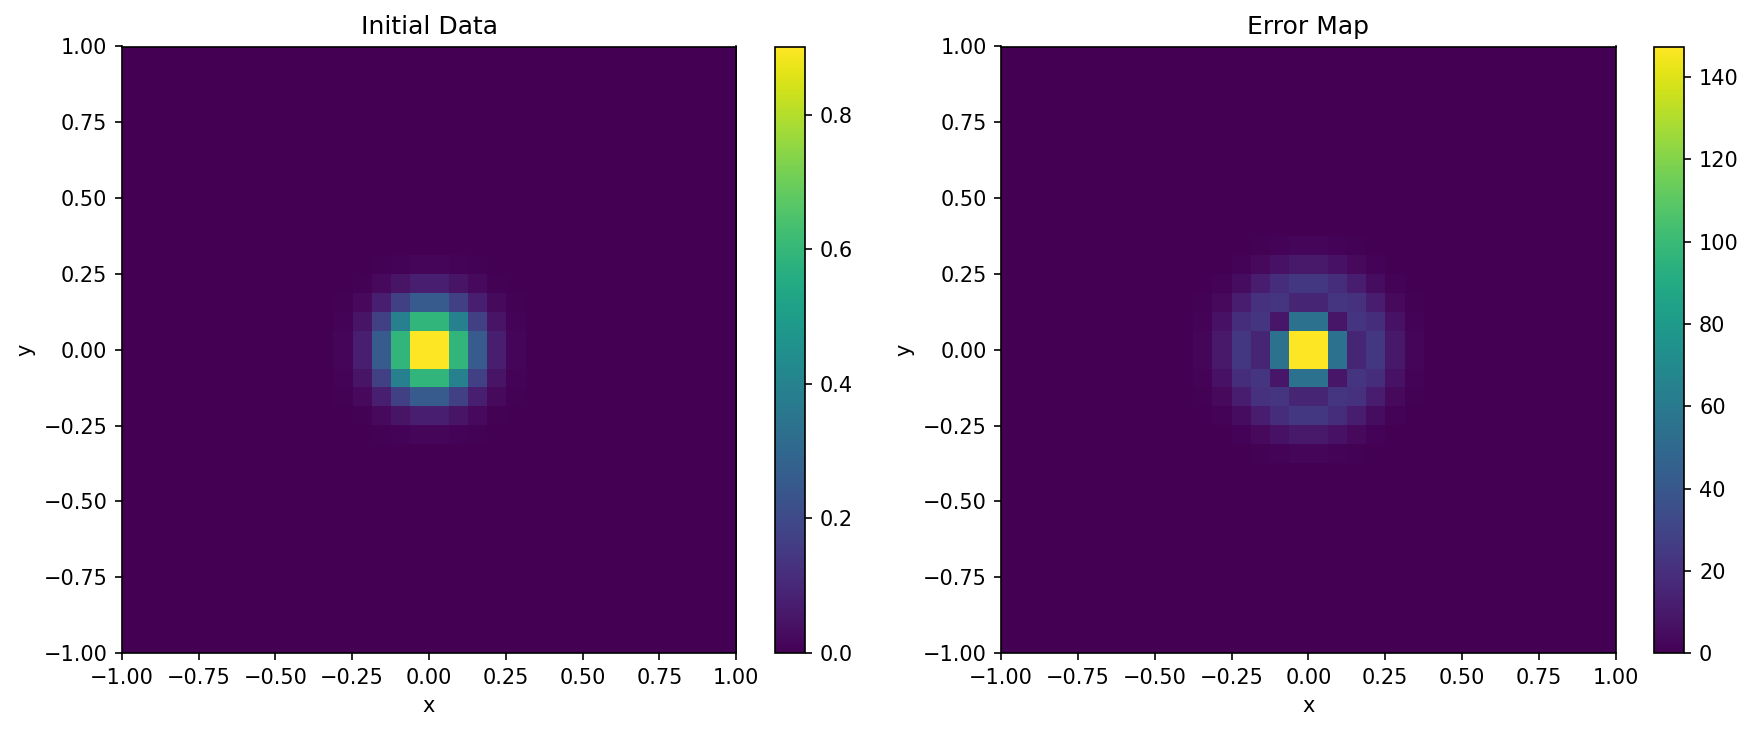
\includegraphics[width=\linewidth]{grid_structure.png}
    \caption{AMR grid hierarchy after 3 refinement levels.}
  \end{subfigure}
  \quad
  \begin{subfigure}[b]{0.45\textwidth}
    \includegraphics[width=\linewidth]{amr_error_plot.png}
    \caption{Error indicator $\eta$ on each patch.}
  \end{subfigure}
  \caption{Demonstration of AMR adapting to high‐curvature regions.}
\end{figure}
\begin{table}[h]
  \centering
  \begin{tabular}{c c c c}
    \hline
    Level $\ell$ & Grid Size $(N_x,N_y)$ & Max $\eta^\ell$ & Residual Norm \\
    \hline
    0 & $(32,\,32)$ & $1.2\times10^{-2}$ & $3.1\times10^{-3}$ \\
    1 & $(64,\,64)$ & $5.6\times10^{-4}$ & $4.2\times10^{-4}$ \\
    2 & $(128,\,128)$ & $1.1\times10^{-4}$ & $9.7\times10^{-5}$ \\
    3 & $(256,\,256)$ & $2.3\times10^{-5}$ & $2.1\times10^{-5}$ \\
    \hline
  \end{tabular}
  \caption{Error and residual norms at successive refinement levels.}
\end{table}

\subsection*{7. Conclusion}
The AMR module significantly reduces computational cost by focusing high resolution only where needed, while achieving second‐order convergence in key observables.  Future work will integrate this AMR layer with full 3+1D matter coupling.

\end{document}
